%# -*- coding: utf-8 -*-
\documentclass{beamer}
\usepackage[bars]{beamerthemetree}
\usetheme{Darmstadt}
%\usecolortheme{lily}
%\usecolortheme{sidebartab}
\usestructuretemplate{\color{structrue}}{}
\beamertemplateshadingbackground{magenta!5}{blue!5}

\usepackage{xeCJK}
\usepackage{mathrsfs}
\usepackage{latexsym}
\setCJKmainfont[BoldFont=SimHei]{SimSun}
\usefonttheme[onlymath]{serif}
\usepackage{moreverb}

\usefonttheme{structurebold}
\usepackage{amsmath,amssymb}

\title{分离逻辑定理证明器的设计与实现}
\author{PB09210183 何春晖 \\ \hfill \\ 导师:冯新宇 教授}
\date{2013年 6月13日}

\begin{document}
\frame{\titlepage}

%\frame{\frametitle{目录}\tableofcontents}
%\AtBeginSection[]
%                  {
%                    \begin{frame}<beamer>
%                      \frametitle{目录}
%                      \tableofcontents[currentsection]
%                    \end{frame}
%                  }
\section{背景}
\begin{frame}[fragile]
  \begin{block}{背景:程序验证}
    \begin{itemize}
    \item 分离逻辑是一种处理可变数据结构的程序逻辑
    \item 为提高验证可信度,要产生机器可检查的证明
    \item 需要一定的自动化
    \end{itemize}
  \end{block}
  \pause
  \begin{block}{现有证明器不能完全满足需要}
    \begin{columns}
      \begin{column}{0.45\textwidth}
        交互式证明器(Coq等):
        \begin{itemize}
        \item 可支持分离逻辑
        \item 证明能够被事后检查
        \item 自动化较差
        \end{itemize}
      \end{column}
      \begin{column}{0.45\textwidth}
        SMT证明器(Z3等):
        \begin{itemize}
        \item 不支持分离逻辑
        \item 证明难以被事后检查
        \item 完全自动化
        \end{itemize}
      \end{column}
    \end{columns}
    分离逻辑原型系统(Smallfoot等):无证明、支持理论不足
  \end{block}
  \pause
  \begin{block}{本文内容}
    试图改进现有系统表达能力、自动化和可信性不平衡的问题。
  \end{block}
\end{frame}

\section{设计}
\begin{frame}[fragile]
  \begin{block}{总体设计}
    \begin{center}
    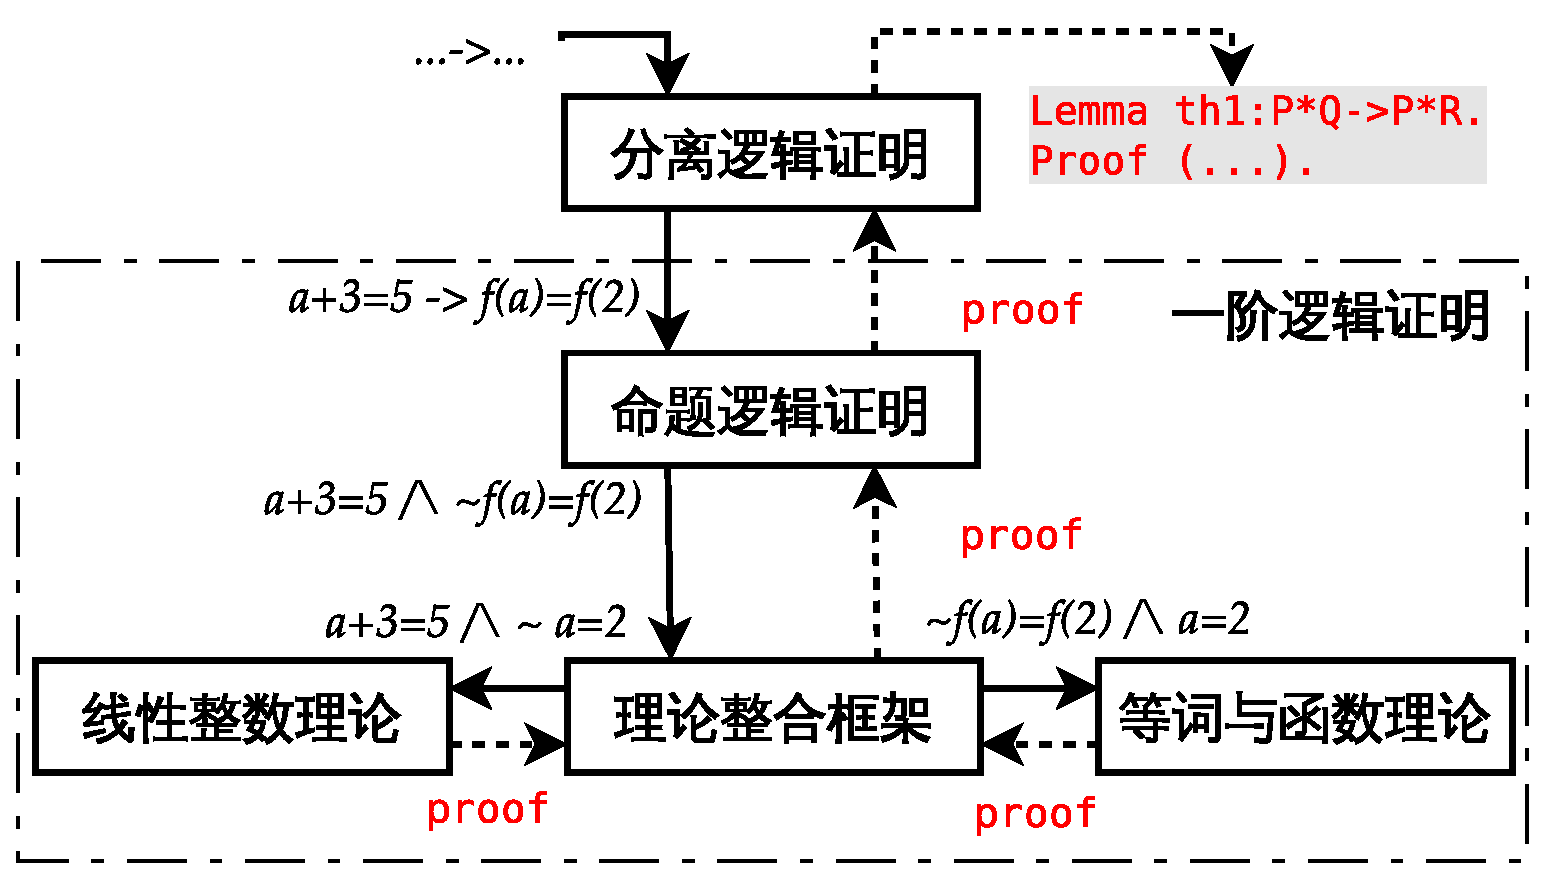
\includegraphics[width=0.8\textwidth]{stru.eps}
    \end{center}
  \end{block}
  \begin{block}{}
    \begin{enumerate}
      \item 主体基于SMT结构(Z3)
      \item 每一步都会生成Coq证明(Coq)
      \item 支持简单的分离逻辑(Smallfoot)
    \end{enumerate}
  \end{block}
\end{frame}

\begin{frame}[fragile]
  \begin{block}{命题逻辑证明}
    \begin{enumerate}
      \item 规范化:将命题的否定转换为CNF范式
      \item SAT求解:寻找可能使命题成假的模型
    \end{enumerate}
  \end{block}
  \begin{block}{}
    \begin{columns}
      
      \begin{column}{0.6\textwidth}
        $$ P \land ( P \rightarrow Q ) \rightarrow Q $$
        \begin{itemize}
        \item 规范化有9种情形
        \item SAT求解基于DPLL决策过程
        \item 成假模型输出给理论求解框架
        \end{itemize}
      \end{column}

      \begin{column}{0.4\textwidth}
        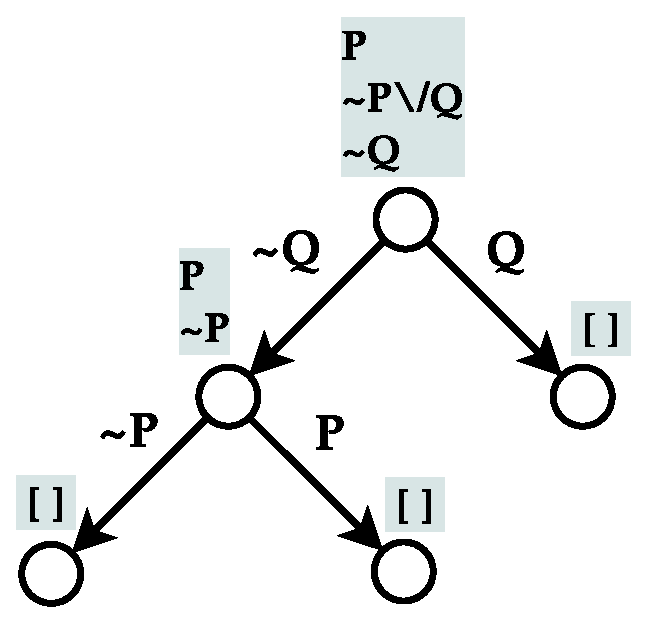
\includegraphics[width=0.85\textwidth]{sat.eps}

        $P \land (\lnot P \lor Q) \land \lnot Q$
      \end{column}

    \end{columns}
  \end{block}
  \begin{block}{}
    $$(P \rightarrow \mathrm{False}) \land (\lnot P \rightarrow \mathrm{False}) \rightarrow \mathrm{False}$$
  \end{block}
\end{frame}

\begin{frame}[fragile]
    \begin{columns}
      
      \begin{column}{0.5\textwidth}
        \begin{block}{等词与函数理论}
          \begin{center}
            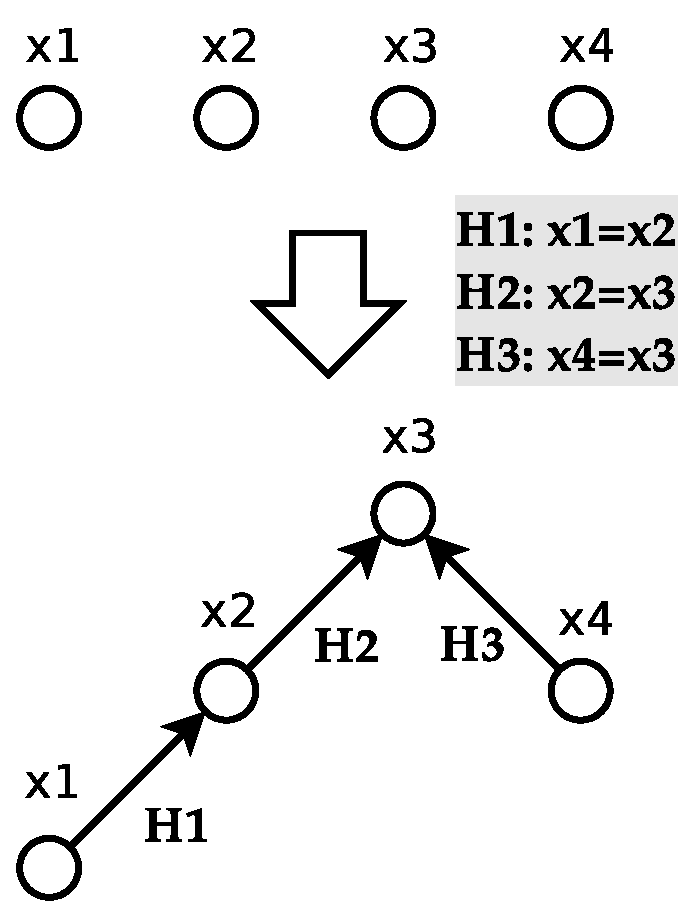
\includegraphics[width=0.65\textwidth]{euf.eps}
          \end{center}
          基于并查集(Union-Find Set)
        \end{block}
      \end{column}

      \begin{column}{0.5\textwidth}
        \begin{block}{线性整数理论}
          \begin{center}
          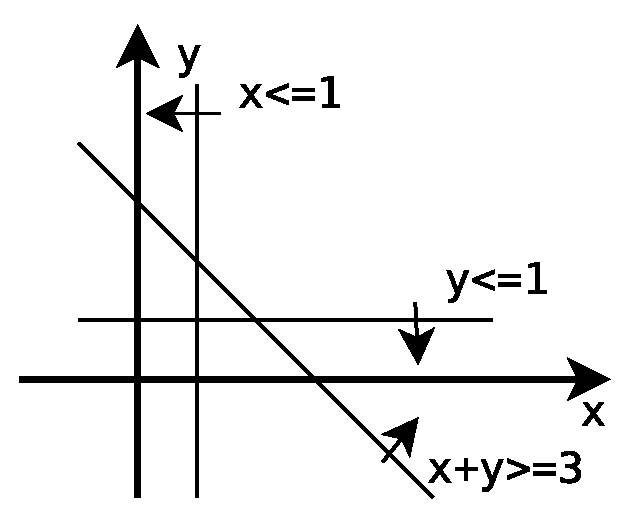
\includegraphics[width=0.7\textwidth]{arith.eps}
          \end{center}
          基于单纯形法(Simplex Method)
        \end{block}
        \begin{block}{理论整合}
          Nelson-Oppen框架
        \end{block}
      \end{column}

    \end{columns}

  \begin{block}{}
    \begin{itemize}
    \item 等词的自反、对称、传递律及函数的等价替换律
    \item $x \leq a \land x > a \rightarrow \mathrm{False}$
    \end{itemize}
  \end{block}
\end{frame}

\begin{frame}[fragile]
  \begin{block}{分离逻辑证明}
    $$ \Pi \land \Sigma \rightarrow \Pi' \land \Sigma' $$
    
    $\Pi$和$\Sigma$分别代表一阶逻辑部分和分离逻辑部分。
  \end{block}
  \begin{columns}
    \begin{column}{0.5\textwidth}
      \begin{block}{分解}
        \begin{eqnarray}
          \vdash & \Pi \land \Pi'' \rightarrow \Pi' \label{struct:eq1}\\
          \vdash & \Pi \land \Sigma \rightarrow \Sigma' \label{struct:eq2}
        \end{eqnarray}

        \ref{struct:eq1}式是纯的一阶逻辑的证明过程。

        \ref{struct:eq2}式是带分离逻辑的证明过程。
      \end{block}
    \end{column}
    \begin{column}{0.5\textwidth}
      \begin{block}{分离逻辑部分}
        frame 规则:
        \begin{center}
        $ P \rightarrow Q \vdash P \ast R \rightarrow Q \ast R$
        \end{center}
        \begin{itemize}
        \item 暂不考虑归纳谓词
        \item 基于frame规则匹配
        \item 分离逻辑在中的Coq定义
        \end{itemize}
      \end{block}
    \end{column}
\end{columns}
\end{frame}

\section{实现}
\begin{frame}[fragile]
  \begin{block}{实现情况}
    \begin{center}
    \includegraphics[width=0.8\textwidth]{strux.eps}
    \end{center}
  \end{block}
  \begin{block}{}
    \begin{enumerate}
    \item 分离逻辑部分还没有实现
    \item 线性整数理论的证明生成借助Coq
    \item 不影响可行性与可信性论证
    \end{enumerate}
  \end{block}
\end{frame}

\begin{frame}[fragile]
\begin{block}{测试}
  单位:秒,精度:0.01秒,有效位数:2位。
    \begin{tabular}{crrrr}
    \hline
    测试内容 & 本文判定 & Coq & Z3 & 本文编译 \\
    \hline
    常见重言式 & 0.01 & 0.06 & <0.01 & 27 \\
    5变量CNF范式 & <0.01 & 0.32 & <0.01 & 0.14 \\
    8变量3-SAT问题 & 0.05 & 超内存 & 0.01 & 110 \\
    线性整数理论 & 0.03 & 0.17 & 0.01 & 3.9 \\
    等词与函数理论 & <0.01 & 0.01 & <0.01 & 0.75 \\
    混合理论 & 0.02 & 0.86 & 0.01 & 2.3 \\
    \hline
  \end{tabular}
\end{block}
\begin{block}{结论}
  \begin{enumerate}
  \item 可行性:单纯判定命题时的性能指标优于Coq,且自动化。
  \item 可信性:输出证明通过Coq验证。
  \item 缺陷:生成证明还不够好,编译时间过长。
  \end{enumerate}
\end{block}
\end{frame}

\section{总结}
\begin{frame}[fragile]
  \begin{block}{设计:在现有系统中作折中}
    \begin{itemize}
      \item 自动化:主体基于SMT结构(Z3)
      \item 可信性:每一步都会生成Coq证明(Coq)
      \item 表达力:支持简单的分离逻辑(Smallfoot)、多理论(Z3)
    \end{itemize}
  \end{block}
\pause
  \begin{block}{实现:一阶逻辑的证明部分}
    \begin{itemize}
    \item 可行性:判定性能优于Coq、自动化
    \item 可信性:输出证明通过Coq验证
    \item 缺陷:生成证明还不够好
    \end{itemize}
  \end{block}
\pause
  \begin{block}{进一步的工作}
    \begin{itemize}
    \item 完善决策过程
    \item 改进证明生成
    \item 实现分离逻辑证明部分
    \end{itemize}
  \end{block}
\end{frame}
\end{document}
